\chapter{Introduction}
\label{introduction}

This dissertation presents a continuum treatment of growth in
biological tissue developed within the context of modern mixture
theory. The crux of this work is a careful examination of the
assumptions underlying continuum thermodynamics under the condition
that multiple interacting species occupy a region of Euclidean space
simultaneously. The formal axiomatic treatment presented derives from
these assumptions, and provides insight into the sequence of
interaction between tissue mechanics, mass transport and biochemical
reactions. A computational formulation built upon the theory is used
to solve a broad class of numerical examples demonstrating several
biophysical aspects of tissue growth.

This initial chapter serves primarily to motivate the research and
provide some context for this work (Section~\ref{background}). It also
briefly articulates the goals of this present investigation and
defines its scope (Section~\ref{goals}), before concluding with an
overview of the topics considered in the remainder of the Dissertation
(Section~\ref{overview}).

\section{Background and motivation}
\label{background}

\textbullet\ This is what growth is and these are the sorts of things
that affect it. (e.g. fig). Describe the current state of the field.

\emph{Growth} involves the addition or depletion of mass in biological
tissue. Growth occurs in combination with
\emph{remodelling}, which is a change in microstructure, and possibly
with \emph{morphogenesis}, which is a change in form in the embryonic
state. The physics of these processes are quite distinct, and for
modelling purposes can, and must, be separated. Our previous work
\citep{growthpaper}, upon which we now seek to build, drew in some
measure from \citet{CowinHegedus:76, EpsteinMaugin:2000}, and
\citet{TaberHumphrey:2001}, and was focused upon a comprehensive
account of the coupling between transport and mechanics. The origins
of this coupling were traced to the balance equations, kinematics and
constitutive relations. A major contribution of that work was the
identification and discussion of several driving forces for transport
that are thermodynamically-consistent, in the sense that specification
of these relations does not violate the Clausius-Duhem dissipation
inequality. 

Recognising the complexity of the system presented (that it is open
with respect to mass and energy, and contains numerous species which
are capable of interacting and inter-converting) and the limitations
of classical  mechanics, additional terms (scalar mass sources/sinks,
vectorial mass fluxes and terms for momentum and energy transfer
between species) are introduced enhancing classical balance laws. The
complex cascades of biochemical reactions are treated in an elementary
fashion, using source-sink terms to govern inter-conversion and mass
fluxes that supply nutrient and remove byproducts.

There have been a number of significant papers on biological growth
and remodelling in the last 7--8 years of which we touch upon some,
whose approaches are either similar to ours in some respects or differ
in important ways. \citet{HumphreyRajagopal:02} provided a
mathematical treatment of \emph{adaptation} in a tissue, which includes 
growth and remodelling in the sense of this paper. The authors
identified adaptation as perhaps the most important mechanical
characteristic of biological tissue. They introduced the notion of evolving
natural configurations to model the state of material deposited at
different instants in time. The treatment of the growth part of the
deformation gradient in this paper bears some resemblance to this
idea, although a detailed development has not been pursued here. The
focus, instead, is on detailing some aspects of the problem that
derive from treatment of the tissue as a porous medium, or as a
mixture of interacting species. \citet{PreziosiFarina:2002} developed an
extension to the classical Darcy's Law to incorporate mass exchanges
between reacting species. This consideration is relevant to growth
problems; however, in our opinion, these issues were subsumed in
\citet{growthpaper}, upon which this paper is based. Many of the ideas
employed here are applicable to tumour growth problems; however, due
to our current focus on tendon, we do not include phenomena
such as angiogenesis and cell migration \citep[see for
  example][]{Brewardetal:2003}. The changes in concentration that
occur with growth tend to cause swelling or contraction of the
tissue. This phenomenon has been accounted for previously by us in fields unrelated to
Biology, using the idea of thermal expansion. See, for
example, \citet{Rao2:00} and \citet{Garikipatietal:01}, which, too,
are probably not the first instances of this idea. In the literature
on biological 
growth this connection was made by \citet{KlischHoger:2003}.

\begin{figure}[!hpt]
\centering
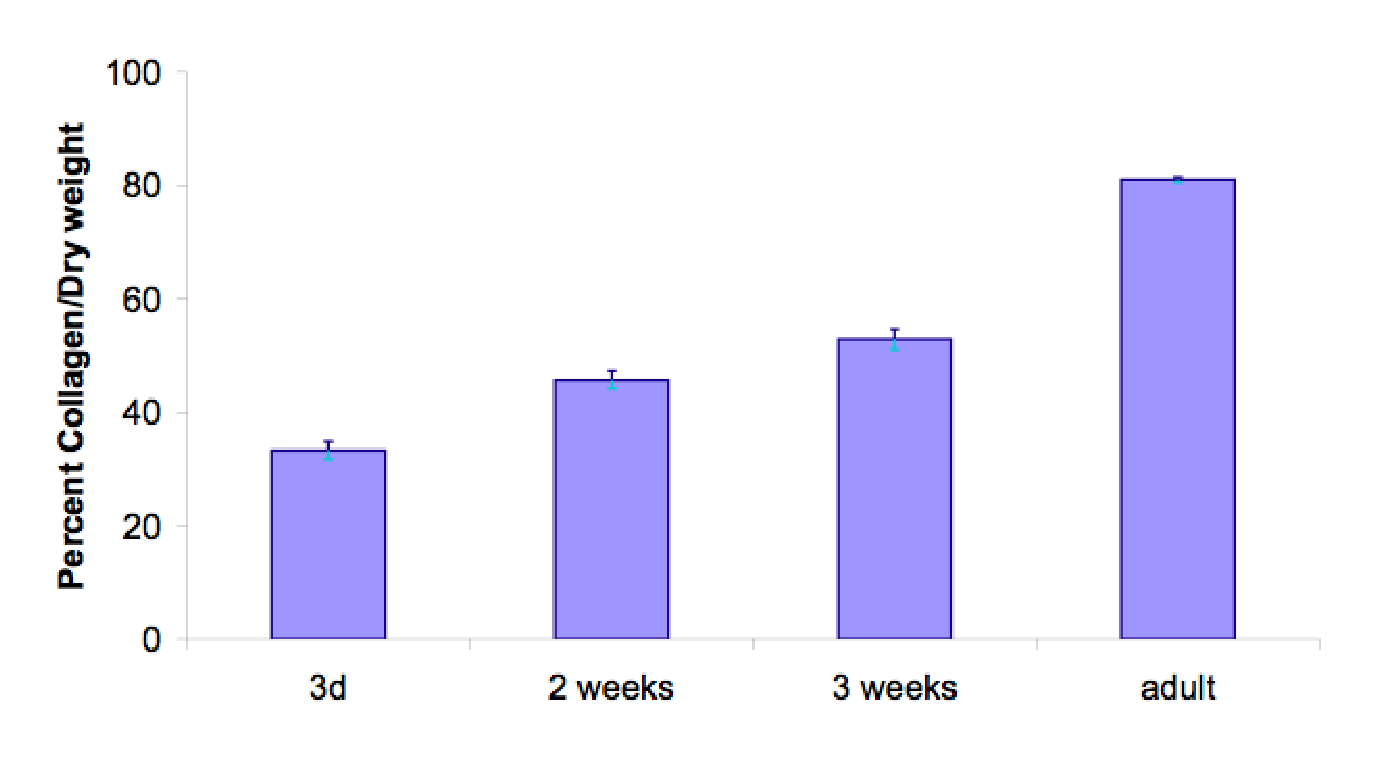
\includegraphics[width=0.8\textwidth]
                {images/experiments/content-evolution} 
\caption{Growth: An increase in collagen concentration with age.}
\label{content-evolution}
\end{figure}

\textbullet\ We're interested in growth in a particular class of tissues, because
of the potential medical implications. Add a few sentences below on
cancer.

Though the formulation is applicable to a large class of open systems
with multiple species potentially participating in reactions, here it is
used to model and predict the response and evolution of one specific
tissue of interest to us, our engineered tendon constructs. These are
functionally immature tendons formed by the self assembly of tendon
fibroblasts {\sl in vitro} \cite{Calve:04}. \mbox{Figure \ref{engconst}}
shows a sample construct 15 days after it has been plated. During the
course of development of this tissue, it undergoes numerous complex
processes, but for the purposes of this growth model, we are focused
on the evolution of concentrations of substances such as collagen (see
\mbox{Figure \ref{collagenamt}}), as well as their dependence on
mechanics. 

There are compelling clinical reasons to study tendons. Tendons
consist mostly of collagen and perhaps provide the simplest
physiologically relevant setting to understand the chemical and
mechanical factors affecting proper collagen deposition. Collagen is
the most important structural component of soft biotissue. Errors in 
collagen deposition cause important types of tissue dysfunction
ranging from {\sl cardiomyopathy} (hypertrophy of collagen makes the
heart too stiff to undergo proper volumetric change) to {\sl
  hypertrophic scarring} in burns (where the morphology of collagen is
whirled rather than aligned in overly stiff scars).

Additionally, there are a large number of musculoskelital injuries
each year which result in damage to soft tissues, including
tendon. For tendons damaged beyond repair, replacement is
necessary. This replacement must incorporate most native properties of
tendon to restore function. However, such transplantation is limited
by the availability of viable autograft, resulting in the use of
synthetic materials which are unable to restore long term function due
to incompatibility. Thus, a need exists for replacements which
incorporate as many native properties as possible, necessitating a
systematic study of engineered tendon.

Perhaps a bit surprisingly the above body of literature, except for
Ambrosi and Mollica (2002), has steered clear of the application to
cancer, despite the obvious centrality of growth and resorption to the
physical modelling of solid tumors. The preference has been for
healthy and pathological growth of bones, and soft tissue. The
literature on cancer modelling in mathematical biology has focused on
time evolution of populations, while ignoring spatial variations (for
example Kuznetsov et al., 1994; d'Onofrio, 2005). Recently, however,
there has been some work on tumor modelling that has included spatial
variations by accounting for mechanical effects, such as Jackson and
Byrne (2002) and the more recent review on cancer dynamics by Byrne et
al. (2006). These works include a multi-species formulation with
reactions, mass transport and mechanics, and are therefore more
aligned with Garikipati et al. (2004) and Sengers et al. (2004).

\textbullet\ But the physics involved in these processes are complex and we began
to focus particularly on the mechanics, since that is our
background. (a) for structural response (b) for figuring out internal
things like fluid flows and transport of species because they are
intimately tied to the biology of growth. (mech is rich in itself fig)

\begin{figure}[!hpt]
\centering
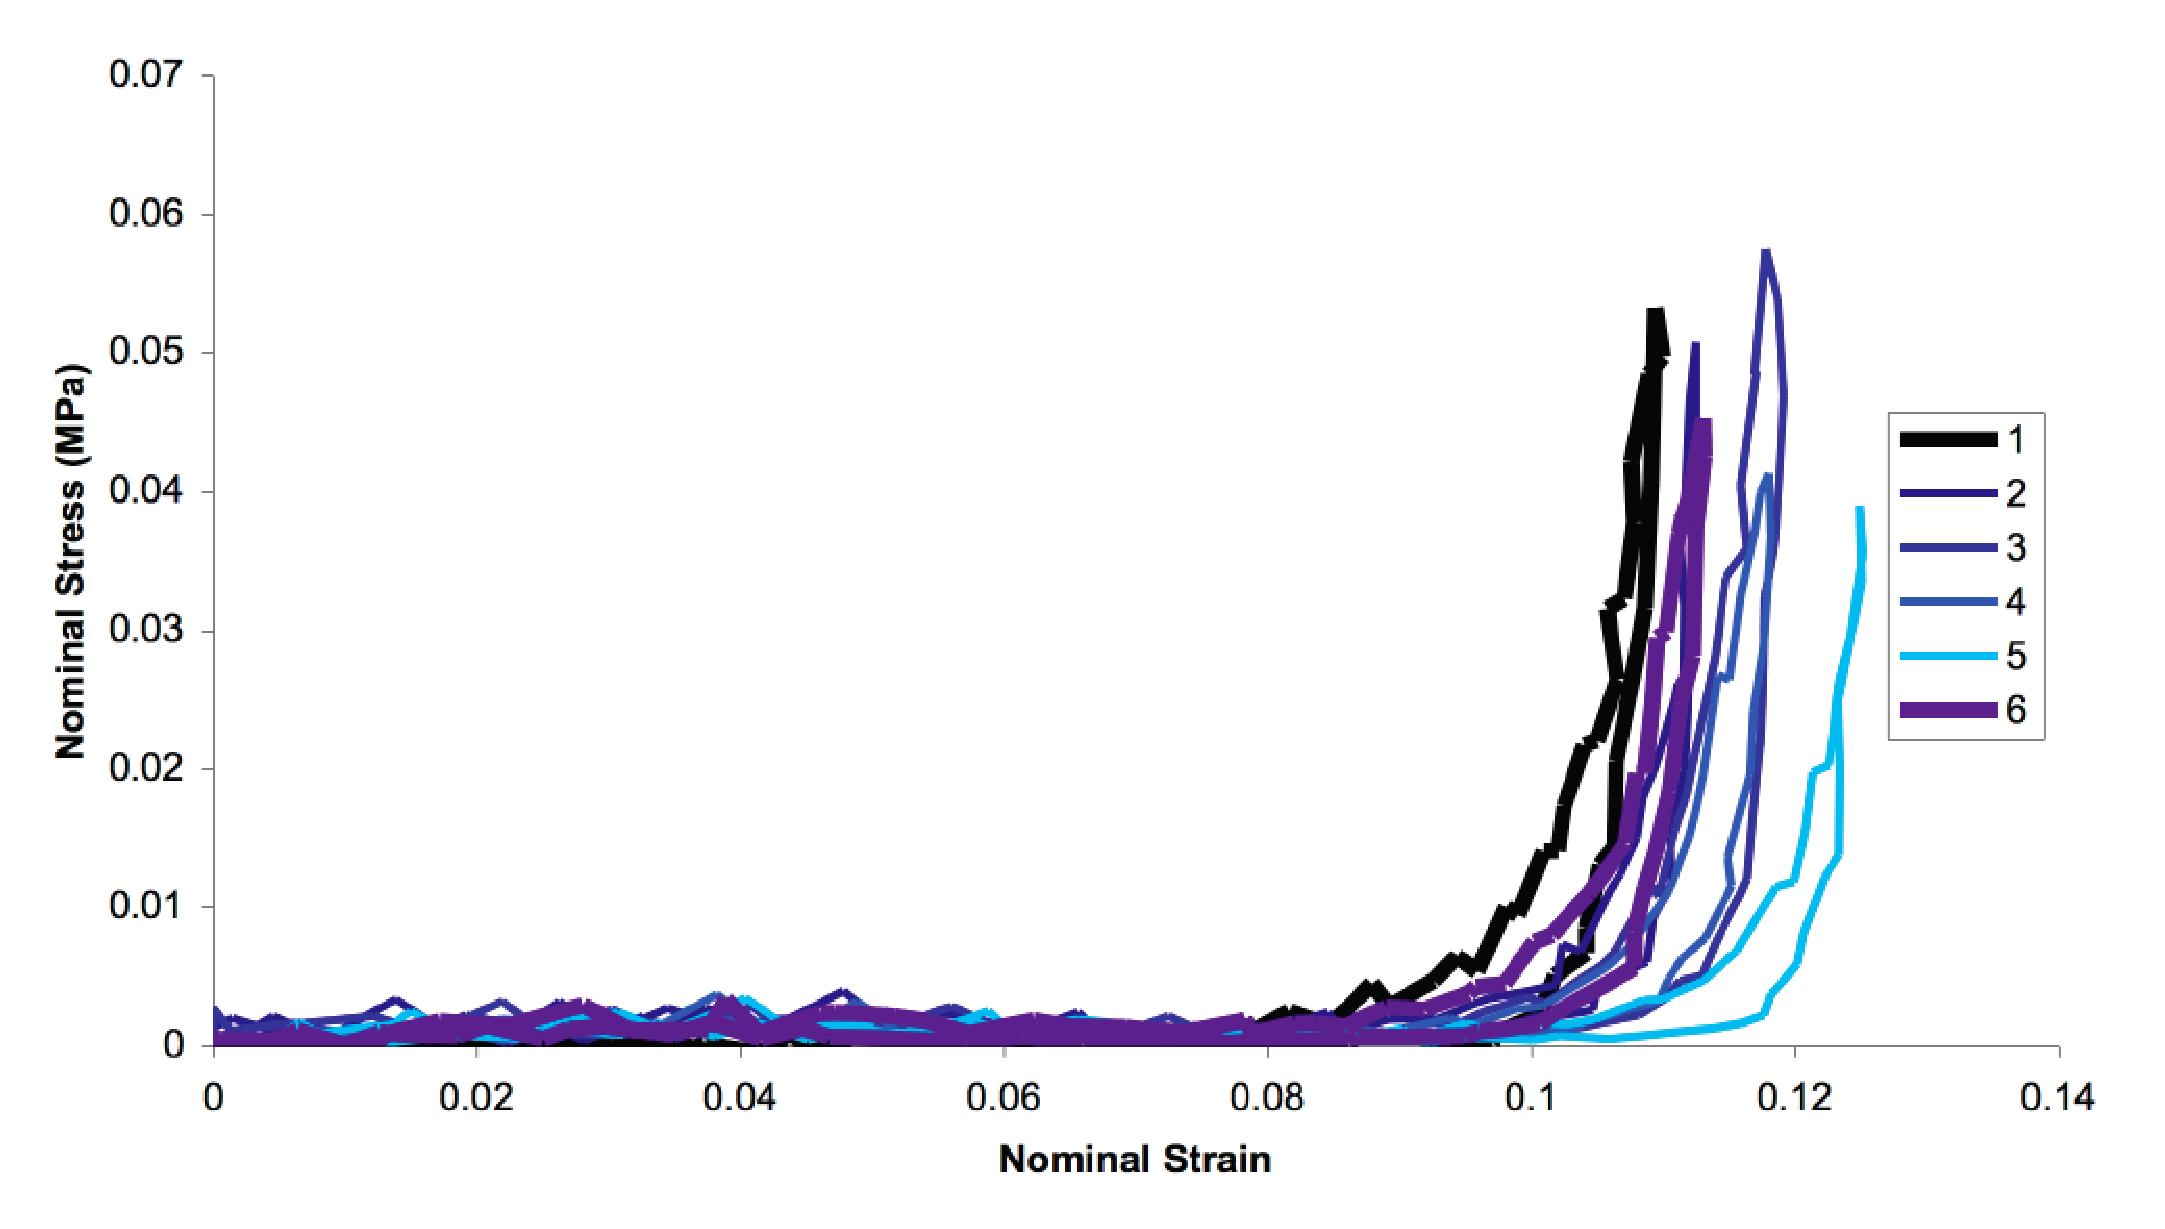
\includegraphics[width=0.8\textwidth]
                {images/experiments/tendon-cyclic-load} 
\caption{Mechanical response of a tendon under repeated cyclic loads.}
\label{tendon-cyclic-load}
\end{figure}

\textbullet\ We're working on a continuum scale because we believe it provides a
reasonable setting for fairly detailed bvp solving without being
bogged down by too much inner detail. The inner detail can be complex
(cite jacks) but they can all be abstracted into a general setting
once the superstructure is fleshed out.

 Additionally,
this is a continuum treatment at a macroscopic scale, rather than at a
cellular or sub-cellular leve.l

\section{Goals and scope}
\label{goals}

The fundamental objectives of this research project are as follows:

\begin{itemize}
\item Formulate a sufficiently general and detailed continuum field
  theory for macroscopic growth, which includes a complete treatment
  of mass transport coupled with mechanics, and implement a
  demonstrative numerical scheme.
\item Make systematic and physiologically relevant modelling choices
  to tailor this general formulation to better represent our current
  tissue of interest, engineered tendon constructs, and use it to
  model and predict the response of the same.
\end{itemize}

Much more work needs to be done to convert this to an actual
helpful computer-aided tool.

The processes of cell proliferation and death, hypertrophy and
atrophy, are complex and involve several cascades of biochemical
reactions. We will treat them in an elementary fashion, using
source/sink terms that govern inter-conversion of species, and the
mass fluxes that supply reactants and remove byproducts. The
treatment will be mathematical; specific constituents will not be
identified with any greater detail than to say that they are
either the tissue's solid phase, the interstitial fluid phase,
precursors of the solid phase (these would include amino acids,
nutrients and enzymes), or byproducts of reactions. We will return
to explicitly incorporate biochemical and cellular processes
within our description of mass transport in a subsequent paper.

\section{An overview}
\label{overview}

\textbullet\ Our first take, 5 years ago, stemmed from classical theories for
the mechanics of solids. Chapter 2 discusses this approach and Chapter
3 computes with it.

\textbullet\ Talk about the contributions of this approach.

In addition to the possibility of multiple species undergoing cascades
of reactions, the full range of driving forces for mass transport,
such as chemical potential gradients, stress gradients, external body
forces such as gravity, has not been systematically treated
previously. Most previous coupling between transport and mechanics has
been through growth-induced residual stress, as described in Section 
\ref{growthdecomp}. As indicated at the outset, this work is aimed at
a complete treatment mass transport, coupled with mechanics, for the
growth problem.

In the present paper, we seek to restrict the range of
physically-admissible models in order to gain greater
physiological relevance for modelling growth in soft biological
tissue. We also include one improvement in the mathematical/numerical treatment:
The advection-diffusion equations for mass transport
require numerical stabilisation in the advection-dominated regime
(the hyperbolic limit). We draw upon the enforcement of the
incompressibility limit for the fluid phase to facilitate this
development.

\textbullet\ 
 The basic problem with this approach was though the mathematical
treatment was consistent and rigorous, modelling choices and viewpoint
choices resulted in having to use quantities like ``deformation
gradient of the fluid.'' While such quantities can be formally
defined, they are not known in practise. Furthermore, they rely on
other assumptions (def grad split) which results in a wide range of
flows and fails to be precise without a lot of work (pedro ponte)

 For a tissue undergoing finite strain, the
  transport equations can be formulated, mathematically, in terms of
  concentrations with respect to either the reference or current
  (deformed) configuration. However, the physics of fluid-tissue
  interactions and the imposition of relevant boundary conditions is
  best understood and represented in the current configuration.

 The modelling of solid-fluid mechanical coupling
  carries strong implications for the stiffness of tissue response,
  the nature of fluid transport, and since nutrients are dissolved in
  the fluid, ultimately for growth. We present upper and lower bounds
  for this problem and computations of coupled boundary value problems with
  these bounds.

\textbullet\ 
 Refining our understanding over these few years, recognising that
there exist many fluid-like phases in the tissue, and they have to be
treated fundamentally different--in terms of their own primitive
variables (velocities, pressure), we revised and further enhanced the
formulation by infusing few years worth of insight gathered about the
system. This discussion is at the heart of Chapter 4.

\textbullet\ 
 Talk about contributions here, and relate it to modern literature.

\textbullet\ 
 With the revised formulation exists the related computational
framework, now written to solve the detailed set of balance equations
and not rely on simplifying assumptions. This seems promising in that
it demonstrates several basic aspects of the physics of these problems
and has been relatively easy to extend to varied classes of problems,
as evidenced by the examples in Chapter 5.

\textbullet\ 
 I believe it's fairly capable, and the scope of the work is general,
from filling tyres (balloon) to modelling visco mechanics arising from
different internal mechanisms, to  the evolution of tumours and wound
healing. The story is brought to a close, along with many ideas on
where else to go in Chapter 6.

As is their very nature, the appendices at the end of this thesis
house topics that while useful, and sometimes interesting, interrupt
the flow of ideas during the main
discourse. Appendix~\ref{additional-proofs} holds additional proofs
which are fairly classical, but they are provided here to ensure that
at least the analytic treatment in this document is fairly
self-contained. And one shouldn't have to run out and grab a text book
on elementary tensor calculus in order to follow
along. Appendix~\ref{supplementary-considerations} contains some
supplementary observations and thought experiments that arose during
the course of the development and refinement of this theory. They are
not all central to the main arguments, but I believe they are quite
interesting.

%% Mention the fact that the boundary conditions we work with in the
%% second formulation is much more natural and amenable to
%% experiments.


%% The principal notion to be borne in mind while developing a
%% continuum formulation for growth is that one is presented with a
%% system that is open with respect to mass. Scalar mass sources and
%% sinks, and vectorial mass fluxes must be considered. A mass source
%% was first introduced in the context of biological growth by
%% \citet{CowinHegedus:76}. The mass flux is a more recent addition
%% of \citet{EpsteinMaugin:2000}, who, however, did not elaborate on
%% the specific nature of the transported species.
%% \citet{KuhlSteinmann:02} also incorporated the mass flux and
%% specified a Fickean diffusive constitutive law for it. In their
%% paper the diffusing species is the material of the tissue itself.
%% The approach to mass transport that is followed in our paper is
%% outlined in the next two paragraphs.

%% In order to be precise about the physiological relevance of our
%% formulation, we have found it appropriate to adopt a different
%% approach from the papers in the preceding paragraph in regard to
%% mass transport. We do not consider mass transport of the material
%% making up any tissue during growth. Instead, it is the nutrients,
%% enzymes and amino acids necessary for growth of tissue, byproducts
%% of metabolic reactions, and the tissue's fluid phase
%% \citep{Swartzetal:99} that undergo diffusion\footnote{We use the
%% terms ``mass transport'' and ``diffusion'' interchangeably.} in
%% our treatment. There do exist certain physiological processes in
%% which cells or the surrounding matrix migrate within a tissue. One
%% such process is observed when leukocytes (white blood cells) such
%% as neutrophils and monocytes are signalled to pass through a
%% capillary wall and are induced, by specific chemical attractors,
%% to migrate to a site of infection. This is the process of
%% chemotaxis \citep{GuytonHall:1996,Vander:2003}. The migrant cells
%% or matrix then participate in some form of cell proliferation or
%% death. Fibroblasts also migrate within the extra cellular matrix
%% during wound healing. A third example is the migration of stem
%% cells to different locations during the embryonic development of
%% an animal. These processes involve very \emph{short range}
%% diffusion, and can be treated by the approach described in this
%% paper. We have chosen to focus upon homeostasis, defined by
%% \citet{Vander:2003} as ``\dots a state of reasonably stable
%% balance betweoen the physiological
%% variables\dots''\footnote{\citet{Vander:2003} go on to say: ``This
%% simple definition cannot give a complete appreciation of what
%% homeostasis truly entails, however. There probably is no such
%% thing as a physiological variable that is constant over long
%% periods of time. In fact, some variables undergo fairly dramatic
%% swings about an average value during the course of a day, yet may
%% still be considered `in balance'. That is because homeostasis is a
%% \emph{dynamic process}, not a static one.''}. Since, to the best
%% of our knowledge, processes of the type just described are not
%% observed during homeostatic tissue growth, we will ignore
%% transport of the solid phase of the tissue.

%% Virtually all biological tissue consists of a solid and fluid
%% phase and can be treated in the context of mixture theory
%% \citep{TruesdellToupin:60,TruesdellNoll:65,BedfordDrumheller:1983}.
%% When growth is of interest, additional species (reactants and
%% byproducts) must be considered as outlined above. The solid phase
%% is an anisotropic composite that is inhomogeneous at microscopic
%% and macroscopic scales. The fluid, being mostly water, may be
%% modelled as incompressible, or compressible with a very large bulk
%% modulus. This level of complexity will be maintained throughout
%% our treatment. The use of mixture theory leads to difficulties
%% associated with partitioning the boundary traction into portions
%% corresponding to each species. \cite{RajagopalWineman:1990},
%% suggested a resolution to this problem that holds in the case of
%% saturated media---a condition that is applicable to soft
%% biological tissue. An alternative is to apply the theory of porous
%% media that grew out of the classical work of Fick and Darcy in the
%% 1800s \citep{Terzaghi:1943,deBoer:2000}. In this approach fluxes
%% are introduced for each species. Since a species that diffuses
%% must do so within some medium, one may think of the various
%% constituents diffusing through the solid phase\footnote{A more
%% sophisticated, and physiologically-correct, description is that
%% the interstitial fluid diffuses relative to the solid phase, while
%% precursors and byproducts of reactants diffuse with respect to the
%% fluid.}. This strategy has been adopted in the present work.

%

% Local Variables:
% TeX-master: "thesis"
% mode: latex
% mode: flyspell
% End:
